\section{Anhang}
\label{sec:Anhang}
\subsection{Messdaten}
\begin{table}[H]
    \centering
    \caption{Gemessener Strom in Abhängigkeit von der Spannung bei $I_{\text{Heiz}} = 2$ und $U_{\text{Heiz}} = 4$ in den linken beiden Spalten und bei $I_{\text{Heiz}} = 2.1$ und $U_{\text{Heiz}} = 4$ in den rechten beiden Spalten.}
    \label{tab:Kennlinie_1_2}
    \begin{tblr}{colspec={c c || c c}}
        \toprule
        $\text{Spannung} \left[\unit{\volt}\right]$ & $\text{Strom} \left[\unit{\milli\ampere}\right]$ & $\text{Spannung} \left[\unit{\volt}\right]$ & $\text{Strom} \left[\unit{\milli\ampere}\right]$ \\
        \midrule  
        10    &  0,013  &   15    &  0,032 \\
        20    &  0,029  &   30    &  0,072 \\
        30    &  0,043  &   40    &  0,096 \\
        40    &  0,050  &   50    &  0,111 \\
        50    &  0,054  &   60    &  0,121 \\
        60    &  0,056  &   70    &  0,121 \\
        70    &  0,056  &   80    &  0,126 \\
        80    &  0,057  &   90    &  0,130 \\
        90    &  0,059  &   100   &  0,133 \\
        100   &  0,059  &   110   &  0,134 \\
        110   &  0,060  &   120   &  0,135 \\
              &         &   130   &  0,136 \\
              &         &   140   &  0,137 \\
              &         &   150   &  0,128 \\
              &         &   160   &  0,139 \\
              &         &   170   &  0,140 \\
              &         &   180   &  0,140 \\
             
        \bottomrule
    \end{tblr}
\end{table}
\begin{table}[H]
    \centering
    \caption{Gemessener Strom in Abhängigkeit von der Spannung bei $I_{\text{Heiz}} = 2,2$ und $U_{\text{Heiz}} = 4,5$ in den linken beiden Spalten und bei $I_{\text{Heiz}} = 2.3$ und $U_{\text{Heiz}} = 5$ in den rechten beiden Spalten.}
    \label{tab:Kennlinie_3_4}
    \begin{tblr}{colspec={c c || c c}}
        \toprule
        $\text{Spannung} \left[\unit{\volt}\right]$ & $\text{Strom} \left[\unit{\milli\ampere}\right]$ & $\text{Spannung} \left[\unit{\volt}\right]$ & $\text{Strom} \left[\unit{\milli\ampere}\right]$\\
        \midrule  
        10      &       0,026 & 15      &       0,052\\
        20      &       0,060 & 30      &       0,128\\
        30      &       0,101 & 45      &       0,214\\
        40      &       0,146 & 60      &       0,306\\
        50      &       0,189 & 75      &       0,402\\
        60      &       0,227 & 90      &       0,491\\
        70      &       0,250 & 105     &       0,557\\
        80      &       0,274 & 120     &       0,609\\
        90      &       0,289 & 135     &       0,644\\
        100     &       0,298 & 150     &       0,667\\
        110     &       0,309 & 165     &       0,683\\
        120     &       0,310 & 180     &       0,694\\
        130     &       0,314 & 195     &       0,702\\
        140     &       0,316 & 210     &       0,709\\
        150     &       0,319 & 225     &       0,714\\
                &             & 240     &       0,719\\
        \bottomrule
    \end{tblr}
\end{table}

\begin{table}[H]
    \centering
    \caption{Gemessener Strom in Abhängigkeit von der Spannung bei $I_{\text{Heiz}} = 2.4$ und $U_{\text{Heiz}} = 5$.}
    \label{tab:Kennlinie_5}
    \begin{tblr}{colspec={c c c c}}
        \toprule
        $\text{Spannung} \left[\unit{\volt}\right]$ & $\text{Strom} \left[\unit{\milli\ampere}\right]$ & $\text{Spannung} \left[\unit{\volt}\right]$ & $\text{Strom} \left[\unit{\milli\ampere}\right]$ \\
        \midrule  
        3       & 0,007 & 54      & 0,299\\
        6       & 0,017 & 57      & 0,322\\
        9       & 0,027 & 60      & 0,352\\
        12      & 0,040 & 65      & 0,400\\
        15      & 0,053 & 70      & 0,441\\
        18      & 0,067 & 75      & 0,492\\
        21      & 0,081 & 80      & 0,535\\
        24      & 0,098 & 85      & 0,576\\
        27      & 0,114 & 90      & 0,626\\
        30      & 0,129 & 110     & 0,786\\
        33      & 0,149 & 130     & 0,930\\
        36      & 0,171 & 150     & 1,053\\
        39      & 0,193 & 170     & 1,158\\
        42      & 0,214 & 190     & 1,238\\
        45      & 0,235 & 210     & 1,292\\
        48      & 0,251 & 230     & 1,330\\
        51      & 0,275 & 250     & 1,356\\
        \bottomrule
    \end{tblr}
\end{table}


\begin{table}[H]
    \centering
    \caption{Gemessener Strom in Abhängigkeit von der Spannung im Anlaufbereich.}
    \label{tab:Anlaufbereich}
    \begin{tblr}{colspec={c c}}
        \toprule
        $\text{Spannung} \left[\unit{\volt}\right]$ & $\text{Strom} \left[\unit{\nano\ampere}\right]$ \\
        \midrule  
        0       & 4,40 \\
        0,05    & 3,00 \\
        0,1     & 2,10 \\
        0,15    & 1,90 \\
        0,2     & 1,45 \\
        0,25    & 1,00 \\
        0,3     & 0,79 \\
        0,4     & 0,40 \\
        0,5     & 0,185 \\
        0,6     & 0,059 \\
        0,65    & 0,014 \\
        \bottomrule
    \end{tblr}
\end{table}
\subsection{Originaldaten}
%
\begin{figure}[H]
  \centering
  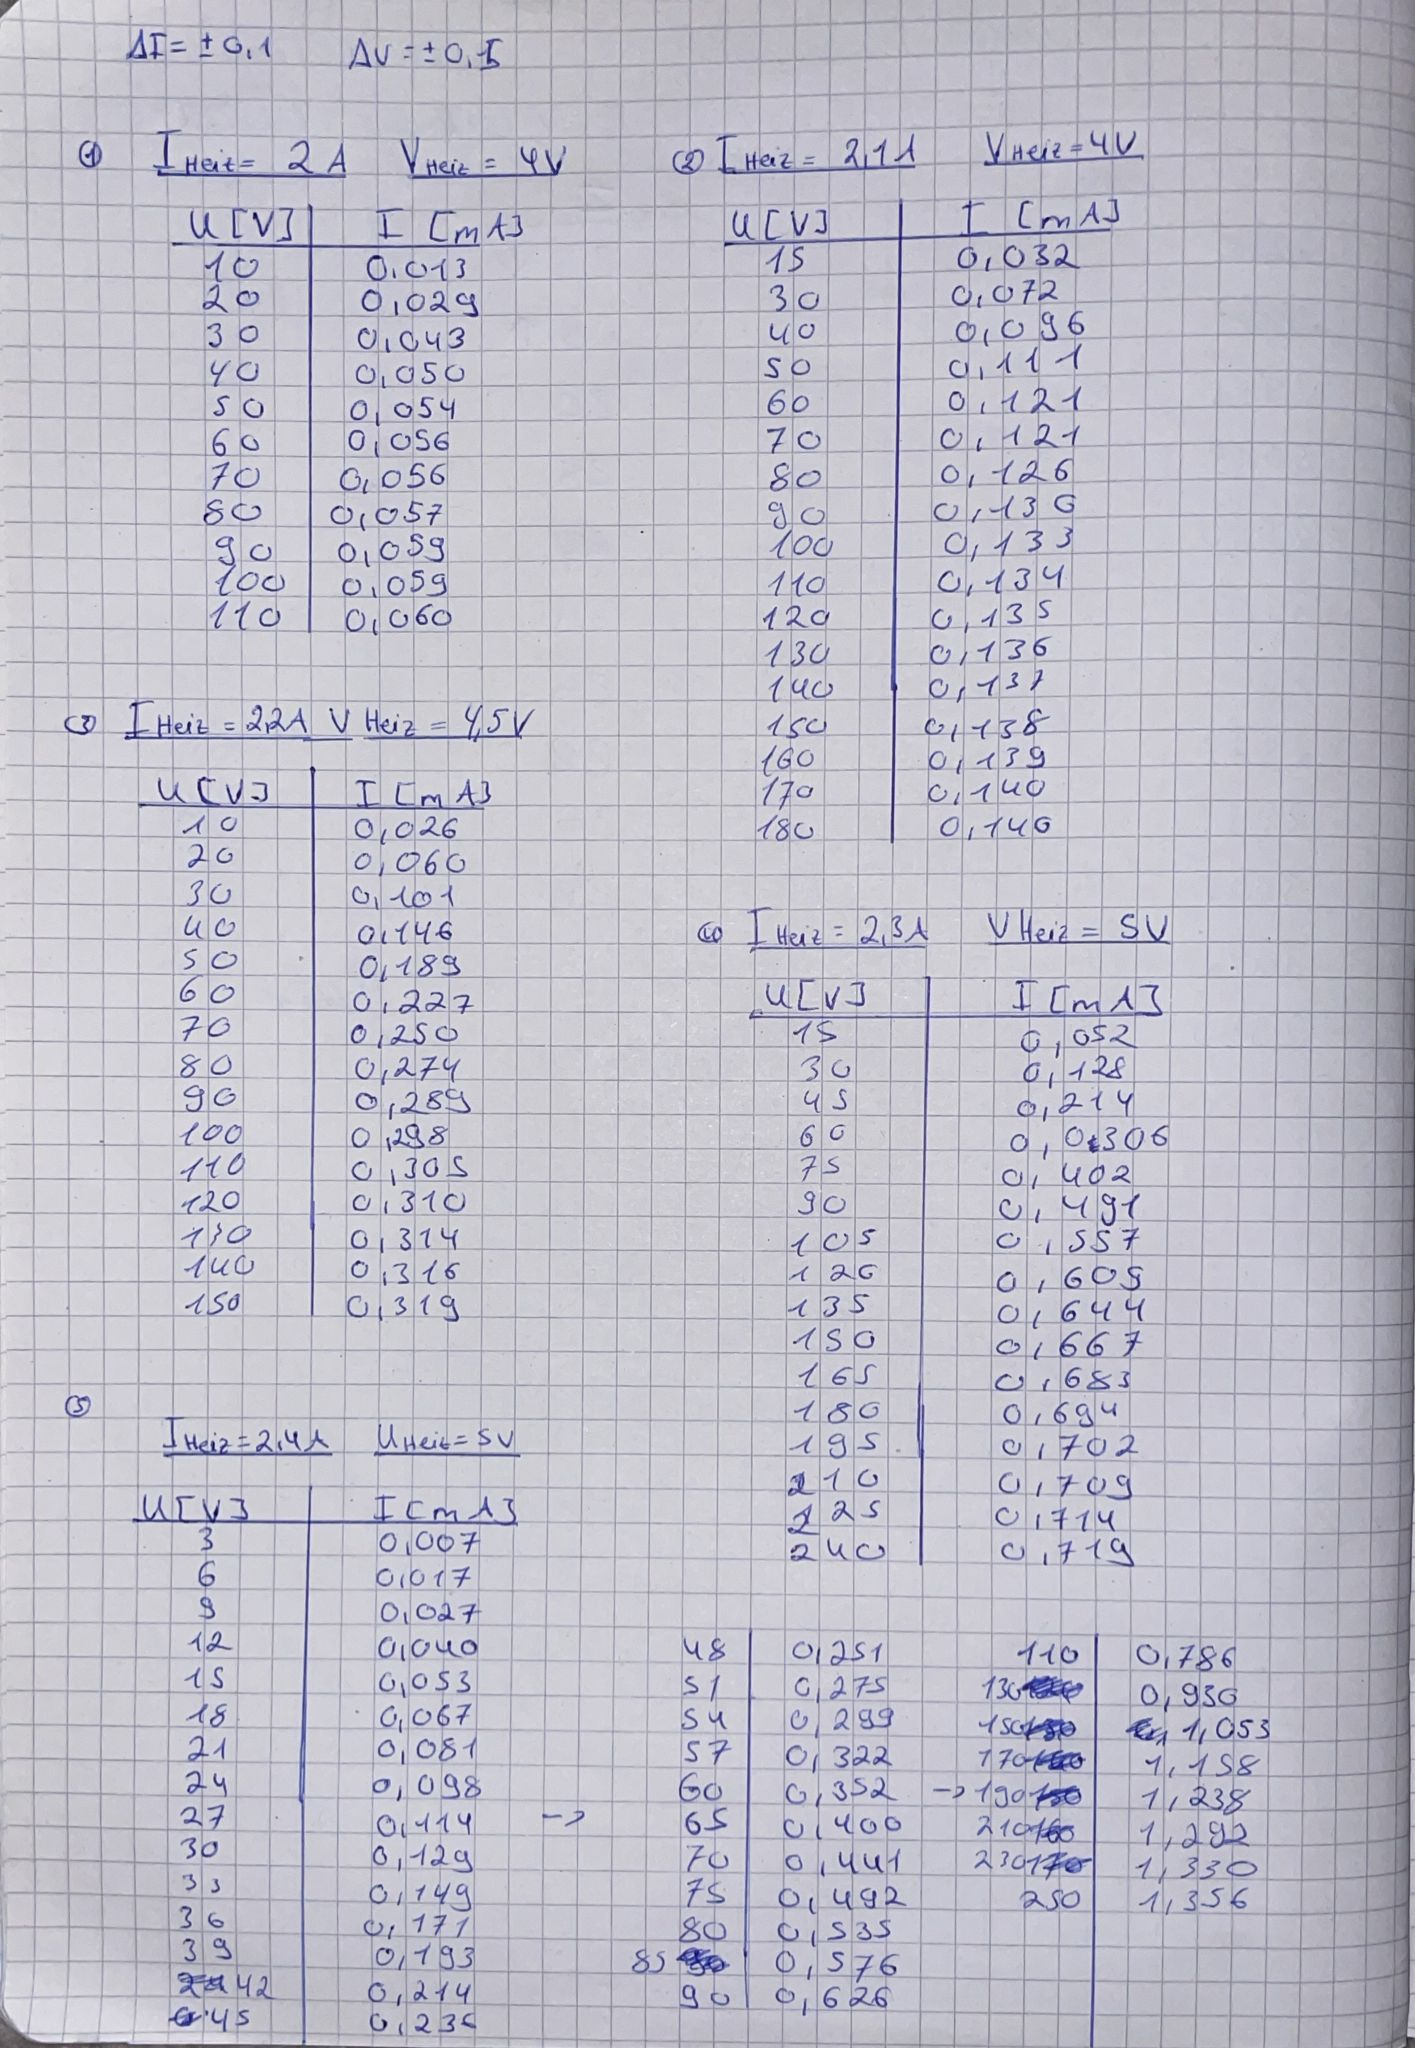
\includegraphics[width=0.90\textwidth]{content/Bilder/Originaldaten_1.jpeg}
  \label{fig:Messungen_1}
\end{figure}
\begin{figure}[H]
  \centering
  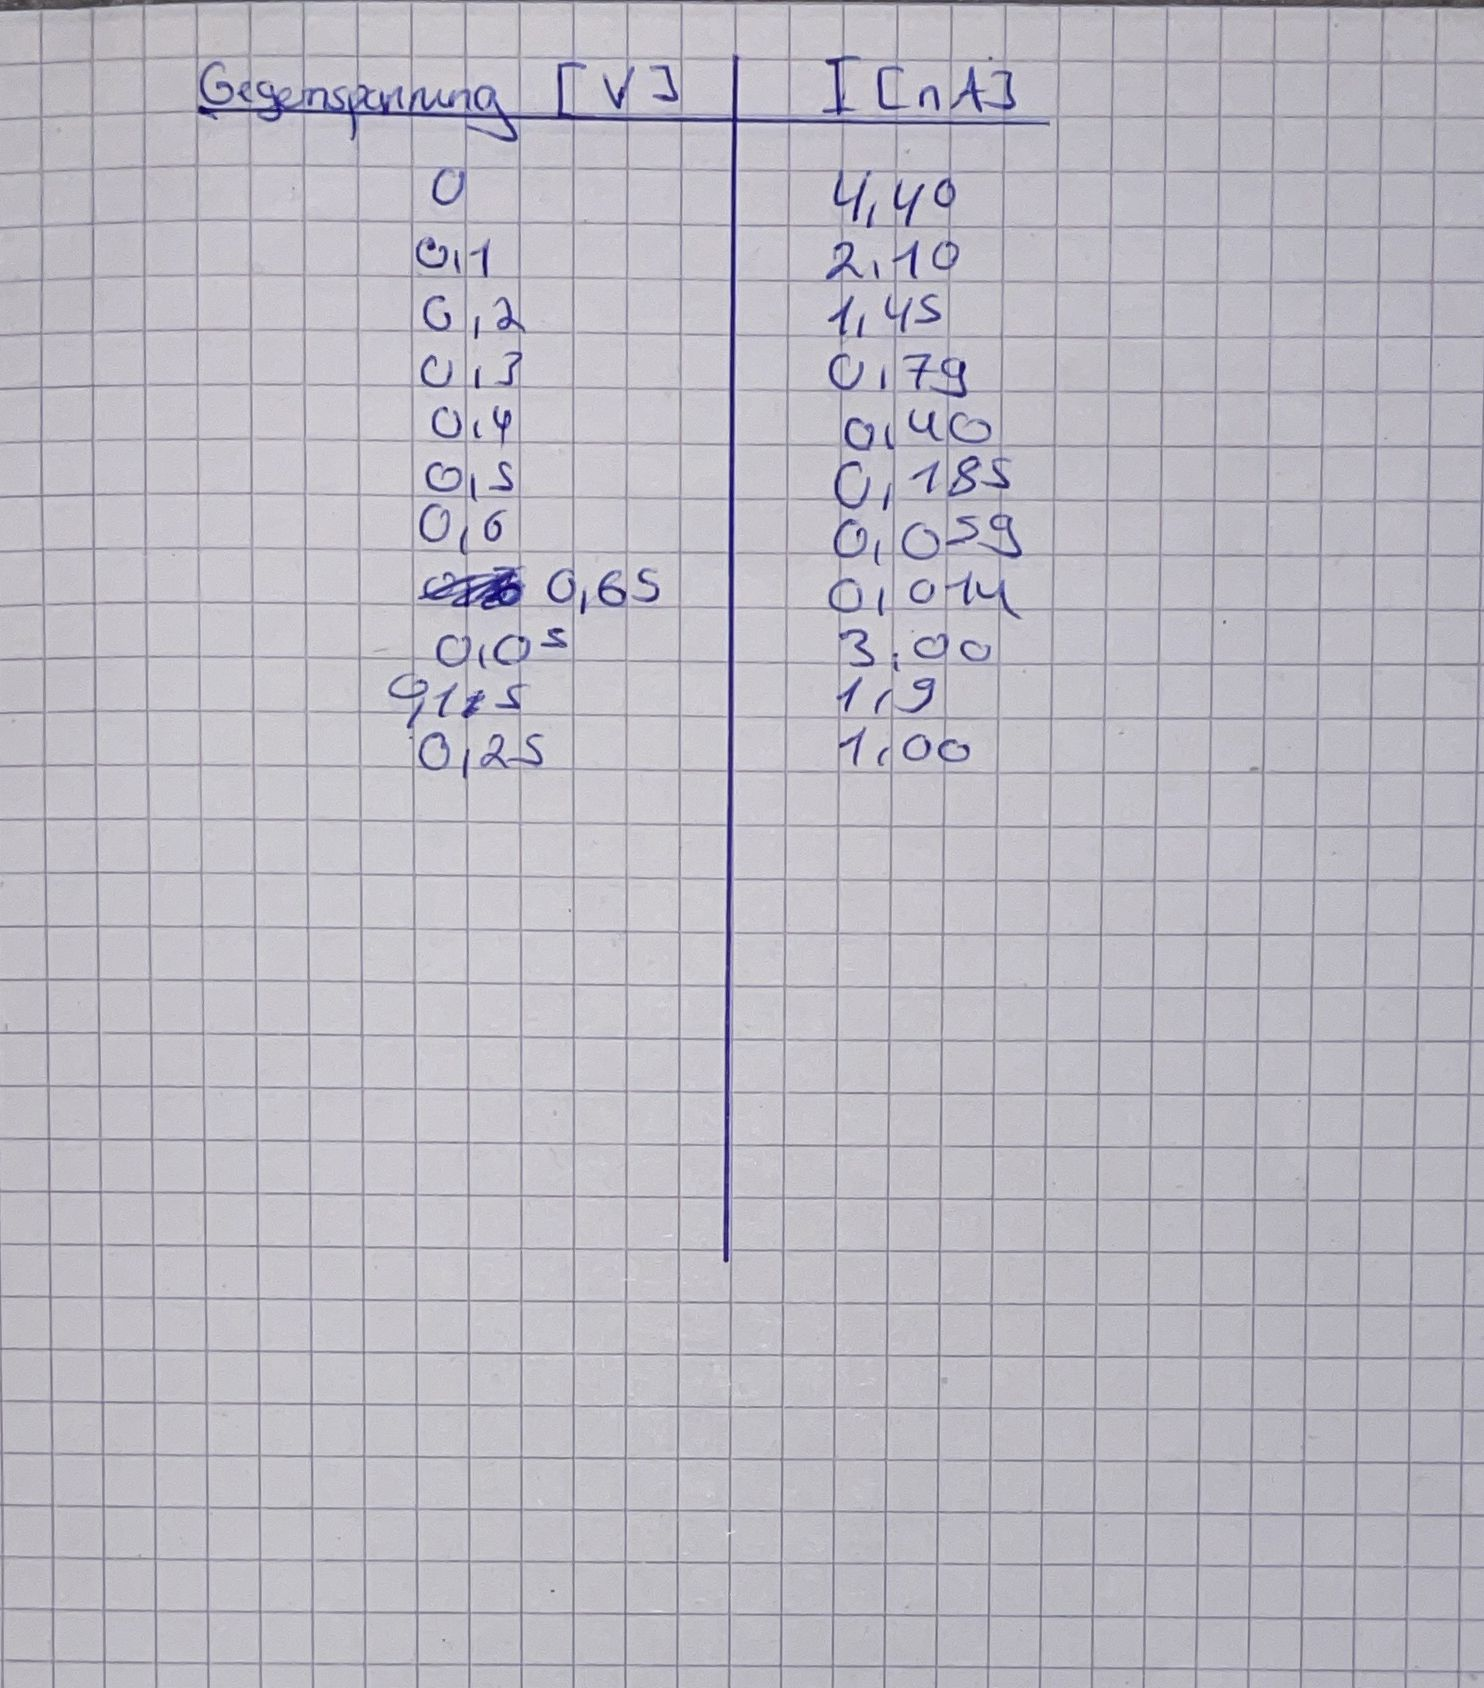
\includegraphics[width=\textwidth]{content/Bilder/Originaldaten_2.jpeg}
  \label{fig:Messungen_2}
\end{figure}
% \end{figure}
% \begin{figure}[H]
%   \centering
%   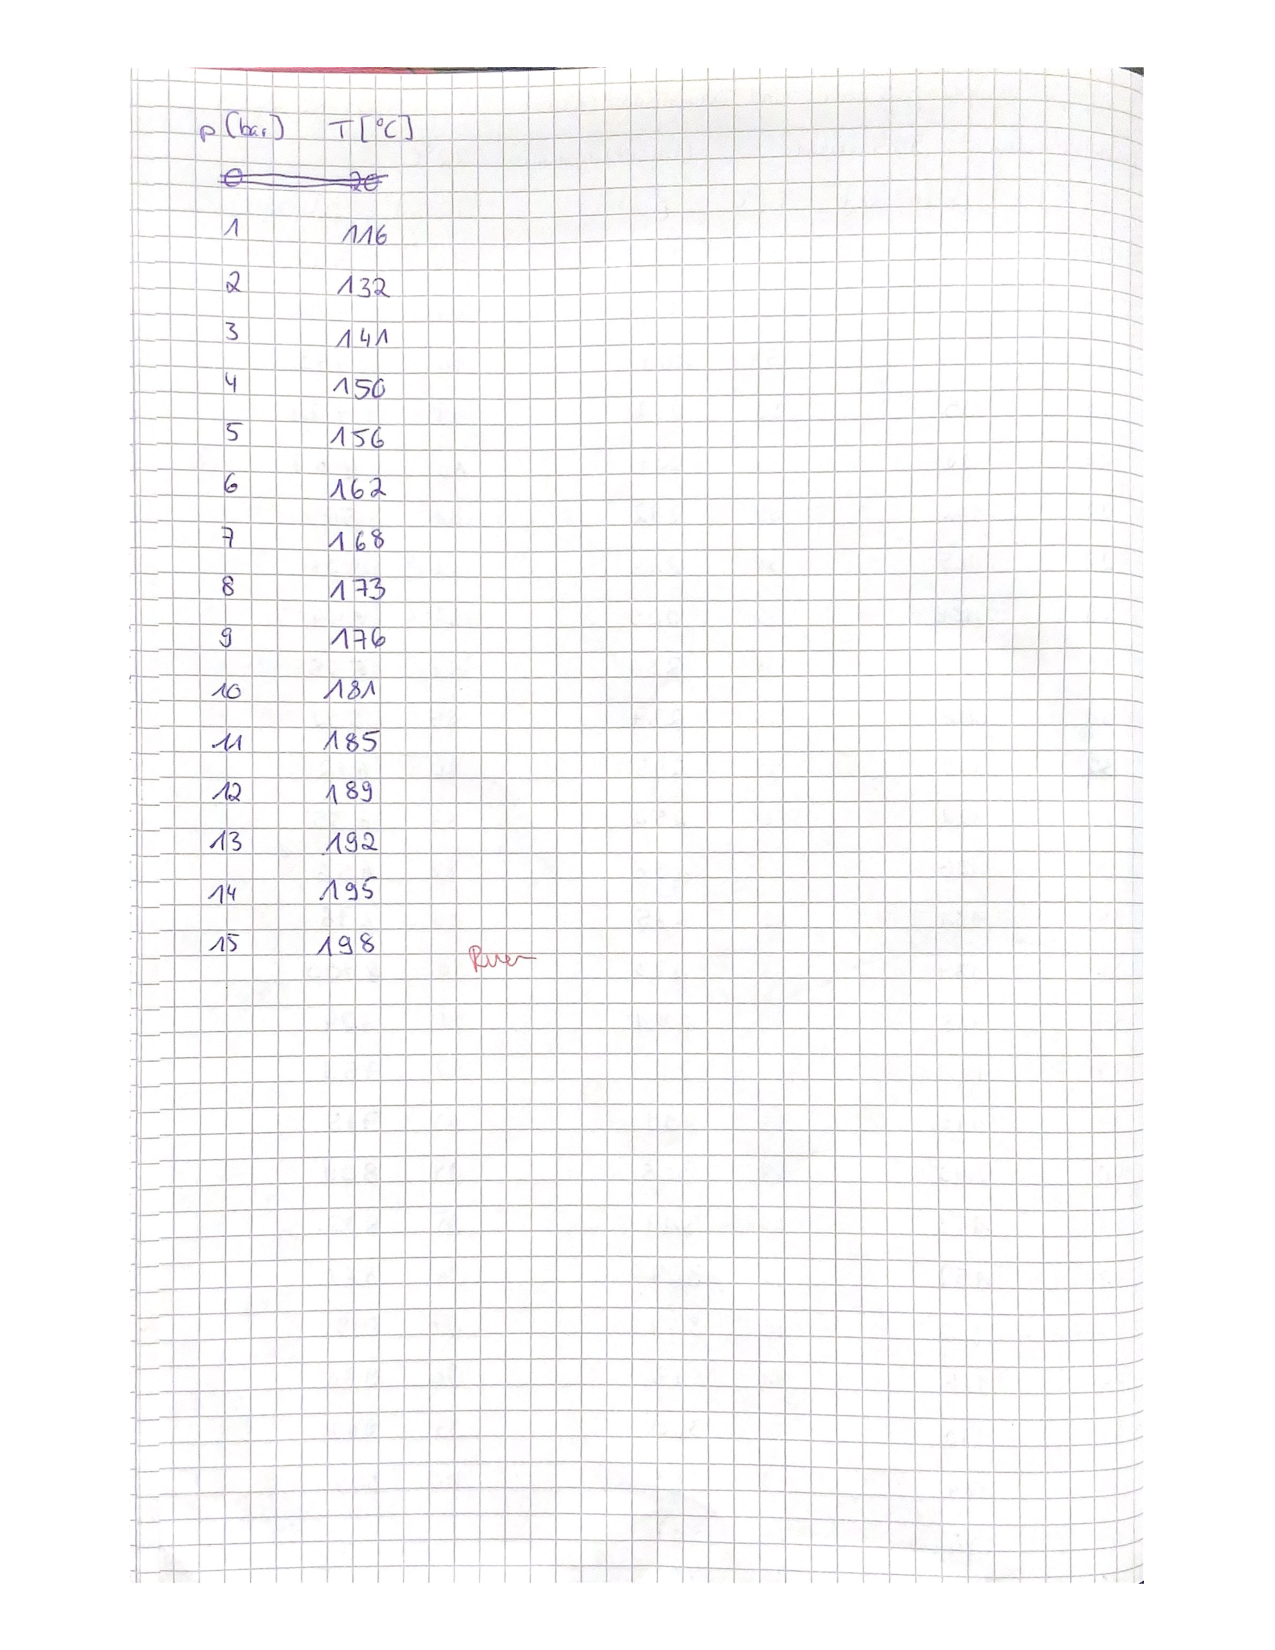
\includegraphics[width=\textwidth]{Messwerte_2.pdf}
%   \label{fig:Messungen_3}
% \end{figure}